\documentclass[../opis-rozwiazania.tex]{subfiles}

\begin{document}

\label{communication}

\subsection{Komunikacja wewnętrzna}
\label{communication:broker}

Komunikacja wewnątrz systemu opiera się na kolejkach opisanych w rozdziale \ref{modules:broker}. W celu uniknięcia wyścigów i utrzymania spójności modelu systemu pomiędzy nadzorcami ustalone zostały następujące zasady:
\begin{itemize}
  \item Nadzorca może zmienić stan systemu jedynie w reakcji na odpowiedź serwera wirtualizacji. Odpowiedzi te wysyłane są do wszystkich nadzorców, dzięki czemu każdy nadzorca ma taki sam model systemu.
  \item Wiadomości przetwarzane są przez serwer wirtualizacji w sposób atomowy. Pojedyncza wiadomość musi zostać w pełni obsłużona zanim program przejdzie do obsługi kolejnej.
  \item Serwer wirtualizacji odpowiada na wiadomości wysyłając nowy stan maszyn. Jeżeli żądanie nie może być spełnione z powodu jego nieaktualności, to serwer na nie nie odpowiada. Wyjątkiem jest żądanie o wysłanie aktualnego stanu maszyn.
  \item Z powodu asynchroniczności wiadomości moduły nie oczekują na odpowiedź. W przypadku nadzorcy dalsze przetwarzanie zostanie uruchomione przez zmianę modelu.
  \item Do monitorowania utrzymania połączenia z brokerem użyty jest mechanizm zwracania wiadomości, które nie mogą zostać dostarczone \parencite{rabbit-unroutable}. Używając go nadzorcy mogą wykryć, kiedy poszczególne serwery wirtualizacji przestaną działać, a serwery wirtualizacji - kiedy wszyscy nadzorcy przestaną działać.
\end{itemize}

Opisane wyżej założenia pozwalają zminimalizować problem hazardu i wyścigów. Jeżeli wiele nadzorców wyśle do serwera wirtualizacji tę samą prośbę (np. o stworzenie sesji na konkretnej maszynie), to z atomowości obsługi sesja zostanie stworzona tylko dla pierwszego z nich. Serwer wirtualizacji wyśle wiadomość o aktualizacji stanu maszyn i zignoruje pozostałe prośby. Nadzorcy otrzymają zmianę stanów, co spowoduje wywołanie odpowiednich procedur. Dla pierwszego będzie to dalsza część procesu tworzenia sesji, a pozostali nadzorcy pozostaną w procesie wyszukiwania maszyny do sesji.

\subsection{Komunikacja zewnętrzna}
\label{communication:api}
Komunikacja aplikacji klienckiej oraz panelu administratora z systemem - nadzorcą - rozwiązana jest za pomocą REST API (\url{https://restfulapi.net/}). W zależności od konfiguracji nadzorcy wiadomości mogą być wysyłane za pomocą protokołu HTTPS, który zapewnia ich szyfrowanie. W tym celu wymagane jest aby na adres, pod którym udostępniony będzie system, wystawiony był odpowiedni certyfikat \parencite{ssl-cert} gwarantujący jego tożsamość.

Poniżej znajduje się zestawienie oraz opis dostępnych endpointów.

\begin{figure}[H]
  \centering
  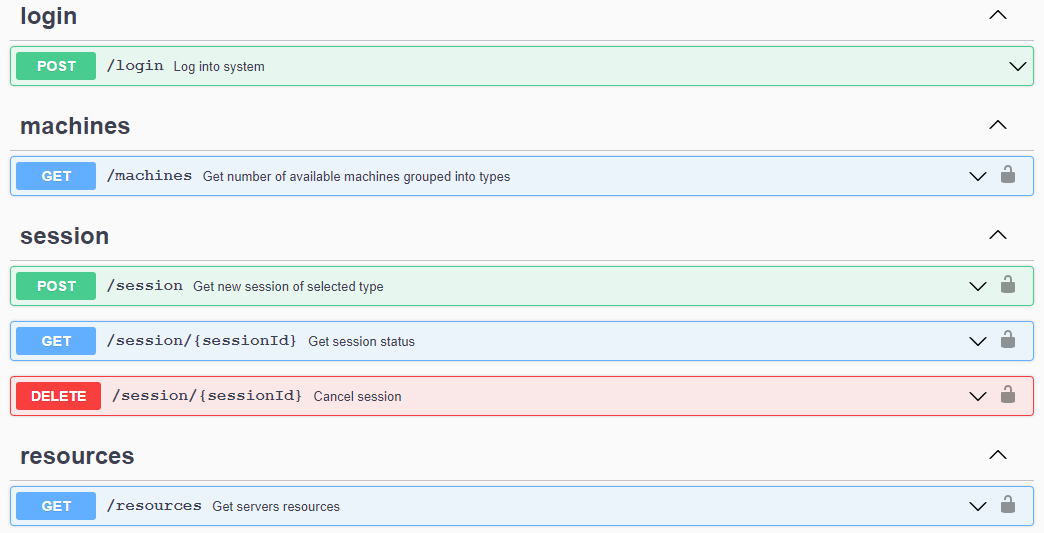
\includegraphics[width=0.9\textwidth]{../api/endpoints.png}
  \caption{Endpointy API}
\end{figure}

\begin{itemize}
  \item Login - służy do logowania do systemu; współdzielony przez aplikację kliencką oraz panel administracyjny. Poprawne zalogowanie zwraca token do dalszej autoryzacji.
  \item Machines - służy do pobierania przez aplikację informacji o typach i ilości dostępnych maszyn. Wymaga autoryzacji poprzez umieszczenie tokenu otrzymanego podczas logowania w odpowiednim nagłówku wiadomości. Dostępny tylko dla użytkowników.
  \item Session - pozwala na wysłanie prośby o uzyskanie sesji, pobranie stanu sesji oraz jej anulowanie. Utworzenie sesji jest możliwe poprzez operację \texttt{POST} z typem maszyny. W odpowiedzi użytkownik dostaje częściowo wypełniony obiekt sesji zawierający id umożliwiające dalsze zapytania. Operacja \texttt{GET} zwraca obiekt sesji z aktualnym stanem. Jeżeli sesja jest gotowa, to zawiera on też adres, z którym należy nawiązać połączenie RDP. \texttt{DELETE} umożliwia anulowanie sesji. Wymaga autoryzacji poprzez umieszczenie tokenu otrzymanego podczas logowania w odpowiednim nagłówku wiadomości. Dostępny tylko dla użytkowników.
  \item Resources - udostępnia informację o zasobach działających serwerów wirtualizacji. Dostępny jedynie dla administratora. Wymaga autoryzacji poprzez umieszczenie tokenu otrzymanego podczas logowania w odpowiednim nagłówku wiadomości.
\end{itemize}

\label{communication:user-broker}

Ważną informacją jaką musi posiadać system jest fakt, czy użytkownik rzeczywiście jest podłączony do maszyny wirtualnej.
System uzyskuje tą informację komunikując się z brokerem wiadomości odpowiedzialnym za komunikację z użytkownikami.
Każda aplikacja kliencka, po uzyskaniu gotowej sesji, tworzy kolejkę o takiej nazwie jak uzyskany identyfikator sesji.
Serwer wirtualizacji sprawdza co jakiś czas czy na końcu kolejki istnieje jakikolwiek konsument.
Gdy użytkownik się rozłączy to aplikacja kliencka usuwa kolejkę, co pozwala serwerowi wykryć zakończenie pracy.

\end{document}